\section{Background}

\begin{multicols}{2}

\subsection{Earth Observation and Remote Sensing}

Remote sensing (RS) refers to the process of acquiring images and data of the planet's surface using a variety of remote sensors in satellite and aerial vehicles (add citations from my prev paper). 
These sensors analyze electromagnetic radiation reflected or emitted from objects on the Earth's surface, which is then processed to extract information about the objects and their properties. 
Besides traditional electro-optical (ie panchromatic and 3-channel RGB images (cite)) modern RS employs a variety of sensors and modalities such as multispectral 
(four or more non-overlapping bands in the electromagnetic spectrum), hyperspectral (more than 100 narrow bands), and even active sensors such as microwave altimeters or Synthetic
Aperture Radar (SAR) that emit their own radiation and measure the reflected signal to ”see” at night and through atmospheric obstructions like clouds and fog (cite myself or refs from prev paper). 
Analysis of source data from these remote sensors must handle a variety of nuanced characteristics of each sensor and the produced data. For our purposes and the scope of this report, we will limit our discussion
to the following characteristics: 

\begin{itemize}
    \item Spatial resolution: The level of detail in an image, typically measured in meters per pixel.
    \item Spectral resolution: The ability of a sensor to distinguish between different wavelengths of light.
    \item Temporal resolution: The frequency at which a sensor captures data over the same location.
    \item Radiometric resolution: The sensitivity of a sensor to detect variations in intensity, often represented by bit depth.
    \item Earth Observation (EO) data types:
        \begin{enumerate}
            \item Raster data: Gridded data representing continuous surfaces.
            \item Vector data: Discrete data represented as points, lines, or polygons.
            \item Time series data: Sequential data capturing changes over time over a specific area.
            \item Geospatial data cubes: Multidimensional arrays combining spatial, temporal, and spectral dimensions.
        \end{enumerate}
\end{itemize}

In the context of data engineering, geospatial data brings several optimization and operations that can ease the process of analyzing large volumes of this type of data.
One of the most relevant concepts for our project is a spatial index 
% A fundamental challenge in RS is the tradeoff that an individual sensor's orbit and design must make between spatial, spectral, and temporal resolution. 


\subsection{Computer Vision}

Computer Vision (CV) is a subfield of Artificial Intelligence and a discipline that deals with the problem of interpreting and extracting meaningful information from images (cite myself or refs from prev paper) 
in a manner similar to human vision. This field has seen significant advancements in recent years, particularly with the rise of deep learning methods and the spread of large, labeled datasets for many applications. 
RS and EO has seen an explosion of interest, publications, and datasets for Deep Learning (DL) methods since 2015\cite{schmitt_datasets_DL_EO_2023}. Relevant CV tasks for our purposes include:

\begin{enumerate}
    \item Scene Classification: Assigning a label to an entire image based on its content (e.g., classifying an image as containing a PV array, rooftop, or vegetation).
    \item Object Detection: Identifying and localizing specific object classes (e.g., PV panels) within an image with (georeferenced) bounding boxes.
    \item Semantic Segmentation: Classifying each pixel in an image into predefined categories (e.g., PV panel array, rooftop, vegetation, background).
    \item Instance Segmentation: Similar to semantic segmentation, but differentiates between \textit{individual} instances (e.g., distinguishing between different PV panel arrays). 
\end{enumerate}

Some relevant CV architectures include Convolutional Neural Networks (CNNs), Vision Transformers (ViTs), Generative Adversarial Networks (GANs), and CNN-Transformer hybrids. 

% - Importance of satellite imagery for monitoring renewable energy infrastructure.
% - Characteristics of PV arrays as seen from space (spectral, spatial).
% - Brief overview of relevant sensor types (multispectral, VHR).

\subsection{STAC}
\label{subsec:stac} % Added label for cross-referencing

A SpatioTemporal Asset Catalog (STAC) is a specification schema that provides a standardized, open, and interoperable way to describe and catalog geospatial information. 
It enables \textbf{efficient searching, discovery, and access} to imagery, sensor data, and other Earth observation (EO) products. 
STAC has emerged as a crucial component in modern geospatial data infrastructure and workflows, addressing the challenges of 
managing and accessing vast volumes of EO data when performing large-scale analysis.

Key features and benefits of STAC include:
\begin{itemize}
    \item \textbf{Standardization}: STAC defines a common language for describing geospatial assets, using JSON to structure metadata. 
    This includes spatial extent (geometry), temporal coverage (datetime), data providers, licensing, and links to the actual data files (assets) and related resources. 
    \item \textbf{Discoverability}: The STAC metadata structure enables powerful search capabilities. 
    Users can query catalogs based on spatial (e.g. single point, or Polygon features) and temporal criteria, as well as other metadata fields like cloud\_cover, making it easier to find relevant data across diverse collections and providers without needing to understand provider-specific APIs.
    \item \textbf{Accessibility}: STAC catalogs typically link directly to the underlying data assets, often hosted in cloud object storage (e.g. AWS S3, Google Cloud Storage). 
    This allows for direct access to data, often in cloud-optimized formats like Cloud-Optimized GeoTIFF (COG), 
    enabling users to stream or process data without downloading entire image strips.
    \item \textbf{Interoperability}: The specification is designed to be extensible, allowing communities to add specific metadata fields relevant to their domain 
    while maintaining core compatibility. This has led to fast and widespread adoption and the development of a rich ecosystem of tools and services that support STAC. 
    \item \textbf{Cloud-Native Focus}: STAC is inherently cloud-native. It facilitates the creation of large-scale, dynamic catalogs of EO data that can be easily accessed and processed in the cloud, reducing data duplication and transfer costs.
\end{itemize}

The STAC specification consists of several core components:
\begin{itemize}
    \item \textbf{Item}: The fundamental unit in STAC, representing a single spatiotemporal asset (e.g., a satellite scene) described by its metadata and links to data files.
    \item \textbf{Collection}: A group of related STAC Items that share common metadata, such as sensor type, processing level, or geographic region.
    \item \textbf{Catalog}: A flexible structure that organizes STAC Collections and Items, often hierarchically, to facilitate browsing and discovery. Catalogs can link to other Catalogs, Collections, or Items.
    \item \textbf{API}: STAC also defines an API specification (STAC API) that provides a \textit{standardized} way to query and serve STAC metadata \textit{over the web}. This allows for dynamic searching and filtering of large catalogs.
\end{itemize}

The shift towards STAC represents a paradigm change from traditional data download workflows to more dynamic, query-driven access. 
Instead of downloading large, monolithic datasets, users can precisely identify and access only the data they need, often processing it in place and at scale in the cloud.
This approach is critical for handling the ever-increasing volume of EO data (hundreds of TB's daily!) and enabling scalable, on-demand geospatial analysis. 
The STAC ecosystem includes a variety of open-source tools that lower the barrier to adoption, such as \texttt{pystac} (Python library for creating and manipulating STAC objects), 
\href{https://radiantearth.github.io/stac-browser/#/external/maxar-opendata.s3.amazonaws.com/events/catalog.json?.language=en}{STAC Browser} (web-based exploration of STAC catalogs), 
and clients for various programming languages.


\subsection{DGGS and H3}
% * Introduction to DGGS concepts.
% * Specifics of H3: hexagonal, hierarchical, indexing capabilities (`h3.geo_to_h3`, `h3.k_ring`, `h3.grid_distance`).
% * Rationale for using H3 as the foundational grid for spatial aggregation and analysis (Li et al., 2024, for grid-based significance thinking; 
% Oje et al., 2025, for context on DGGS performance, even if HierGP is adaptive).

Traditional geospatial data representation relies heavily on Coordinate Reference Systems (CRS) that project the Earth's curved surface onto a 2D plane.
While widely used, these projections inherently introduce distortions in area, shape, distance, or direction, particularly when analyzing data at global scales or geographically diverse regions. 
Furthermore, \texit{integrating data from various sources with different CRSs can be complex and error-prone}. Discrete Global Grid Systems (DGGS) have emerged as a modern paradigm to address these 
limitations by providing a standardized framework for \textbf{spatially indexing and analyzing global data} \cite{ESRI_DGGS_Intro_2023}.

A DGGS is a spatial reference system that partitions the Earth's surface into a hierarchical tessellation of regular, uniquely identifiable cells. 
Key characteristics of DGGS, as outlined by the Open Geospatial Consortium (OGC) DGGS Abstract Specification \cite{OGC_DGGS_Spec}, include:
\begin{itemize}
    \item \textbf{Cellular Tessellation:} The globe is divided into a mesh of cells, commonly using regular polygons like hexagons, triangles, or squares. \textit{Hexagonal cells are often favored due to their inherent uniform adjacency} 
    (all neighbors are equidistant from the cell center, for regular hexagons) and reduced orientation bias compared to square grids \cite{XDGGS_Kmoch_2024}.
    \item \textbf{Hierarchy and Refinement:} DGGS cells are organized in a \textit{multi-resolution hierarchy}. Cells at a coarser resolution level can be perfectly subdivided into a fixed number of smaller cells at finer resolutions. 
    This hierarchical structure is fundamental for \textit{multi-scale analysis and efficient data aggregation or disaggregation}.
    \item \textbf{Unique Identifiers:} Each cell at every resolution level is assigned a unique identifier (cell ID). This indexing system allows for \textit{efficient data retrieval, querying, and spatial operations based on cell IDs rather than individual or sets of geographic coordinates}.
    \item \textbf{Approximately Equal Area:} Many DGGS aim for cells that represent $\sim$equal areas on the Earth's surface at any given resolution level. This property is crucial for accurate statistical analysis and \textit{comparisons across different geographic regions}.
\end{itemize}

The primary advantage of DGGS is that it \textbf{can provide a globally consistent and performant spatial framework}, minimizing the distortions inherent in traditional map projections and simplifying the integration of diverse geospatial datasets \cite{ESRI_DGGS_Intro_2023, XDGGS_Kmoch_2024}. 
This makes DGGS particularly well-suited for \textit{large-scale environmental modeling, Earth observation data analysis, and global data fusion tasks}.
While various DGGS implementations exist, each with different cell shapes (e.g., triangles, squares, hexagons) and projection bases, hexagonal grids have gained popularity for several reasons. 
Hexagons are the most compact regular polygon to tile a plane, offering higher packing density. 
They also exhibit uniform adjacency, meaning all six neighbors of a central hexagon are equidistant (for regular hexagons) and share edges of the same length, which simplifies neighborhood calculations and reduces orientation bias compared to square grids \cite{XDGGS_Kmoch_2024}.

\textbf{Uber's H3} (2018) is a prominent open-source DGGS that utilizes a hexagonal, hierarchical grid system. 
It divides the Earth into base cells projected onto the faces of an icosahedron, which are then recursively subdivided into finer hexagonal cells across 16 resolution levels\cite{H3_Overview}. 
H3 provides efficient functions for:
\begin{itemize}
    \item Indexing geographic coordinates to cell IDs (e.g., \texttt{h3.latlng\_to\_cell()}). As discussed previously, this operation is approximately O(1) for a single point due to its direct geometric transformations and fixed series of bounded computations.
    \item Aggregating adjacent data points within H3 cells (e.g., \texttt{h3.cell\_to\_geo\_boundary()} to retrieve the vertices of a cell that contains a set of points).
    \item Hierarchical multi-resolution traversal (e.g., finding parent or child cells).
    \item Neighborhood analysis (e.g., \texttt{h3.k\_ring()} to find cells within a certain grid distance).
    \item Calculating grid distance between cells (e.g., \texttt{h3.grid\_distance()}), which measures the minimum number of cell traversals.
\end{itemize}

For this project, H3 is adopted as the foundational DGGS for several reasons. Firstly, its hierarchical indexing allows for flexible aggregation of Photovoltaic (PV) Point-of-Interest (PoI) data into discrete spatial units (H3 cells) at an appropriate resolution. 
This aligns with the grid-based significance mapping concept explored by Li et al. (2024) for optimizing \textit{future} Earth observation tasks\cite{Li_H3_EO_planning_2024}, although here \textit{we instead adapt it for analyzing historical/archival data}. 
Secondly, the consistent grid structure and defined neighborhood relationships are naturally conducive to graph-based spatial clustering, where \textbf{H3 cells become nodes in a Minimum Spanning Tree (MST)}. 
The \texttt{h3.grid\_distance} function provides a natural and computationally efficient metric for defining proximity between these H3 cell nodes. 
While spatio-temporal and dynamically-adaptive grid systems like HierGP (cite Oje et al., 2025) \cite{Oje_HierGP_ST_2025} and others offer dynamic partitioning based on data characteristics and demonstrate strong performance in certain benchmarks, H3's 
second-place performance in that same publication, global consistency, well-defined hierarchy, and, particularly, mature software tooling make it a robust choice for developing a standardized analytical framework for our research. 
The unique cell IDs provided by H3 also facilitate efficient data management and linkage between PV locations, derived clusters, and corresponding STAC assets as we'll describe in our Algorithms section.

\end{multicols}

\begin{figure}[h!htbp]
    \centering
    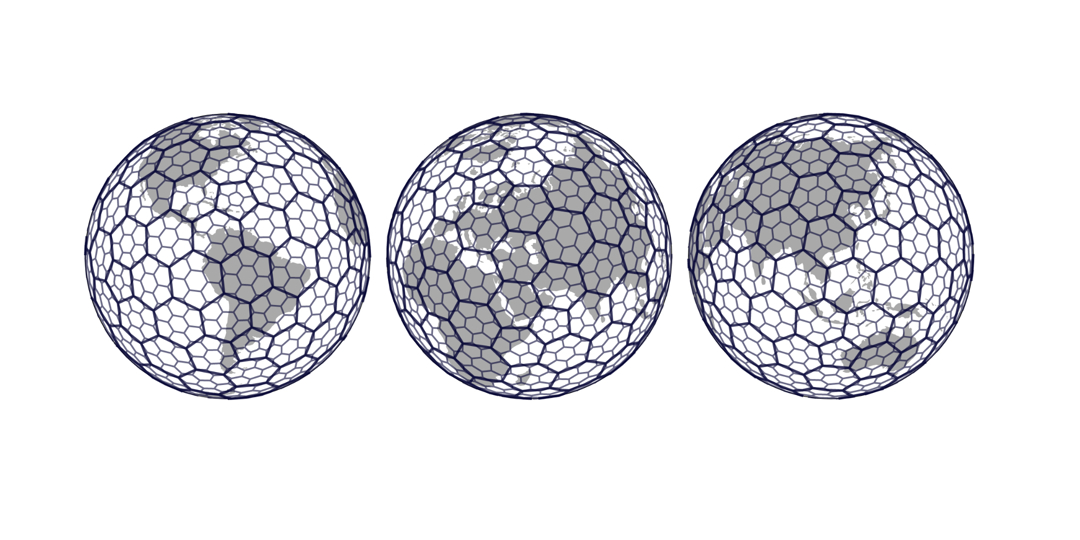
\includegraphics[width=\textwidth]{./report/assets/figures/Uber-H3-globe.png} % should load relative to the main.tex file
    \caption{Illustration of Uber's H3 hexagonal hierarchical spatial index. The image shows the icosahedron base projection and progressive refinement into smaller hexagonal cells across different resolution levels. Source: Uber Engineering Blog.}
    \label{fig:h3_illustration}
\end{figure}

\begin{multicols}{2}

\subsection{Hierarchical-Spatial Clustering}
% * Concept of MSTs in graph theory.
% * Application of MSTs in clustering: identifying natural groupings by cutting edges.
% * Advantages for spatial data: ability to find clusters of arbitrary shapes (Gagolewski et al., 2023).
Spatial Clustering groups data points based on their spatial proximity. 
Hierarchical clustering methods group data points into a tree-like structure of clusters, which is particularly useful for understanding multi-scale patterns in data. 
Hierarchical-Spatial clustering combines both concepts, creating a hierarchy of clusters based on spatial relationships between data points and is particularly useful for analyzing \textit{large-scale geospatial data}.
Minimum Spanning Trees offer a powerful and versatile approach to achieve this.

\subsubsection{Fundamentals of MST-based Clustering}
A Minimum Spanning Tree (MST) of \textit{a connected, undirected graph is an acyclic subgraph that connects all vertices} (data points) with the minimum possible total edge weight. 
In the context of clustering, edge weights typically represent distances or dissimilarities between data points. As noted by Zaslavskiy et al. in "Clustering with Minimum Spanning Trees: How good can it be?"\cite{gagolewski_MST_Clustering_how_good_2024}, 
MST's provide some key properties and advantages for hierarchical-spatial clustering including:
\begin{itemize}
    \item \textbf{Natural Cluster Representation:} An MST for $n$ points always has $n-1$ edges. Removing $k-1$ of the longest or most inconsistent edges from an MST partitions the graph into $k$ connected components, which can be interpreted as $k$ distinct clusters.
    \item \textbf{Detection of Arbitrary Cluster Shapes:} Unlike methods like K-means that assume convex clusters, MST-based approaches can effectively identify clusters of varying densities and arbitrary shapes.
    \item \textbf{No Strong a priori Assumptions:} MST clustering does not require prior knowledge of the number of clusters or strong assumptions about the data distribution.
    \item \textbf{Algorithmic Foundation:} MSTs serve as a foundation for various clustering algorithms, including single-linkage, divisive, and agglomerative hierarchical clustering methods.
\end{itemize}

Classical algorithms for MST construction include \textit{Borůvka's}, \textit{Prim's (Jarník's)}, and \textit{Kruskal's} algorithms, with complexities generally ranging from $O(m \log n)$ to $O(n^2)$ for dense graphs 
(where $n$ is the number of vertices and $m$ is the number of edges). The authors highlight that MST-based methods can outperform popular parametric approaches in benchmarks and can generate a whole hierarchy of clusters efficiently once the MST is computed.

\subsection{Research Gaps and Contribution Goals}
    \begin{enumerate}
        \item Measure performance impact of SOTA Computer Vision architectures [CCOM6120] (e.g. ViT, Swin, CNN-Transformer hybrids) currently lacking in most recent publications and compare to established segmentation baselines (e.g. UNet, FPN, PAN, etc.)
        \item Regional, and global surveys are limited to large-scale farms using medium resolution sensors ($\sim10m$/pixel). On the other hand, studies using VHR aerial imagery usually only have coverage for local, city-scale surveys. We will use open access catalogs from VHR MSI sensors, 
        primarily from Maxar and Sentinel2, and other STAC archives to as the source for a data pipeline that will generate a large-scale global dataset of PV installations and \textbf{design algorithms for efficiently retrieving, storing, and processing this data at scale} [CCOM6050]. 
        The resulting dataset will be used as training data for CV models that can be used to perform a global survey of PV installations that includes both large-scale commerical and utility-scale ``solar farms'' and smaller-scale distributed rooftop PV systems.
        \item Almost all notable studies (with the exception of (cite GloSoFarID)) exclusively use RGB image bands. Measure impact of use of PV-specific spectral indices\cite{He_universal_pv_spectral_index_2024} and specifically the benefits of including NIR + SWIR bands available in Maxar sensors [CCOM6050]. 
        \item Develop a solution that consciously tackles the challenges identified in \cite{Hu_solar_array_pitfalls_2022} for evaluating and performing comparisons of different remote sensing solar array assessment methodologies 
        (\textit{distribution drift, test data quality, level of spatial-aggregation, and proprietary data}) [Thesis].
    \end{enumerate}


\end{multicols}
